\documentclass[11pt,a4paper]{book}

\usepackage{Appunti}

\begin{document}
\title{Docker and Kubernetes: The Complete Guide}
\author{Jacopo De Angelis}
\maketitle

\pagebreak
\tableofcontents
\pagebreak

\chapter{Perchè usare docker e cos'è?}
Docker si prefigge di permettere di passare un software senza doversi preoccupare di dipendenze o altro.

\textbf{Immagine}: un singolo file con tutte le dipendenze e le configurazioni richieste per lanciare un programma.

\textbf{Container}: istanza di un'immagine. 

Il docker client ci permette di interfacciarci con il docker server, un programma col quale non ci interfacciamo direttamente ma è un processo che lavora dietro le quinte.

\chapter{Manipolazione dei container}
\section{docker run}
\emph{\textbf{docker run $<$nome immagine$>$}}: lancia il programma all'interno del programma.

\emph{\textbf{docker run $<$nome immagine$>$ $<$comando$>$}}: all'interno di un'immagine viene lanciato il comando specificato e non quello di default. Nel caso il comando non fosse presente all'interno delle cartelle verrà mostrato un messaggio d'errore.

\begin{figure}[h!]
	\begin{center}
		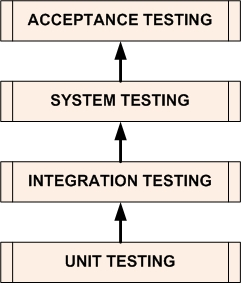
\includegraphics[scale=0.5]{img/002.jpg}
		\caption{Docker run}
		\label{fig: 002}
	\end{center}
\end{figure}

Quando viene lanciato run viene creato un container. 

\section{docker ps}
Tutti i container possono essere mostrati tramite \emph{\textbf{docker ps}}, se vogliamo vedere anche quelli che sono stati terminati in passato allora lanciamo \emph{\textbf{docker ps --all}}. Se vogliamo lanciare un comando relativo ad uno specifico container allora dovremo utilizzare il suo ID o il suo nome.

\begin{figure}[h!]
	\begin{center}
		
\includegraphics[scale=0.5]{img/001.jpg}
		\caption{Docker ps}
		\label{fig: 001}
	\end{center}
\end{figure}

\section{docker run = docker create + docker start}
\emph{\textbf{docker run}} in realtà deriva dall'unione di due comandi: \emph{\textbf{docker create}} e \emph{\textbf{docker start}}; col primo comando semplicemente prepariamo il container, preparandone le risorse.

\emph{\textbf{docker create}} restituisce un ID che può essere usato tramite \emph{\textbf{docker start}}. \emph{\textbf{docker start $<$id$>$}} semplicemente restituirà nuovamente l'id ma avviserà che il container sarà attivato, \emph{\textbf{docker start -a $<$id$>$}} eseguirà anche il comando interno al container.

\begin{figure}[h!]
	\begin{center}
		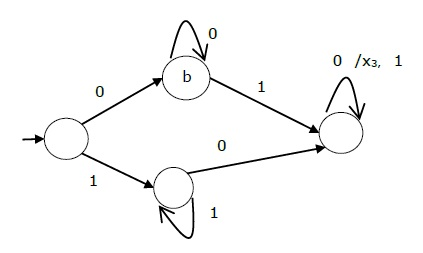
\includegraphics[scale=0.6]{img/003.jpg}
		\caption{docker create e docker start}
		\label{fig: 003}
	\end{center}
\end{figure}

Quando un container è stato spento non vuole dire che non possa essere riavviato, semplicemente dovremo usare \emph{\textbf{docker start -a $<$id$>$}} dove l'id è quello del container spento, così verrà rieseguito il comando eseguito precedentemente.

\section{Eliminazione e terminazione di un container}
\emph{\textbf{docker system prune}} rimuove tutti i container spenti, tutti i network inutilizzati, tutte le immagini non usate e la cache.

\emph{\textbf{docker logs $<$container id$>$}} permette di recuperare tutti i log da un container. \emph{docker logs} non fa ripartire un container, ne recupera solo i log.
\begin{figure}[h!]
	\begin{center}
		
\includegraphics[scale=0.6]{img/005.jpg}
		\caption{docker logs}
		\label{fig: 005}
	\end{center}
\end{figure}

\emph{\textbf{docker stop $<$container id$>$}} stoppa un container mandando un comando di terminazione del segnale per il container (SIGTERM), questo vuole dire che ci verrà restituito un segnale che potremo usare per fare partire altri comandi. Nel caso il container non termini entro 10 secondi verrà mandato un SIGKILL.

\emph{\textbf{docker kill $<$container id$>$}} stoppa un container mandando un comando di terminazione definitiva per il container (SIGKILL), questo vuole dire che appena viene lanciato non c'è niente che possa essere fatto dopo in risposta.

\section{Agire con un container}
Se avviamo un container in docker e poi proviamo a lanciare dei comandi per interagire con esso dall'esterno come se nulla fosse otterremmo un errore, questo deriva dal fatto che le risorse del container sono accessibili solo da dentro il container. Infatti come si vede dall'immagine \ref{fig: 006}, all'interno di docker è stato lanciato un server di redis ma se provassimo ad avviare una connessione a redis dall'esterno direttamente otterremmo un errore nel quale ci viene detto che redis non è attivo.
\begin{figure}[h!]
	\begin{center}
		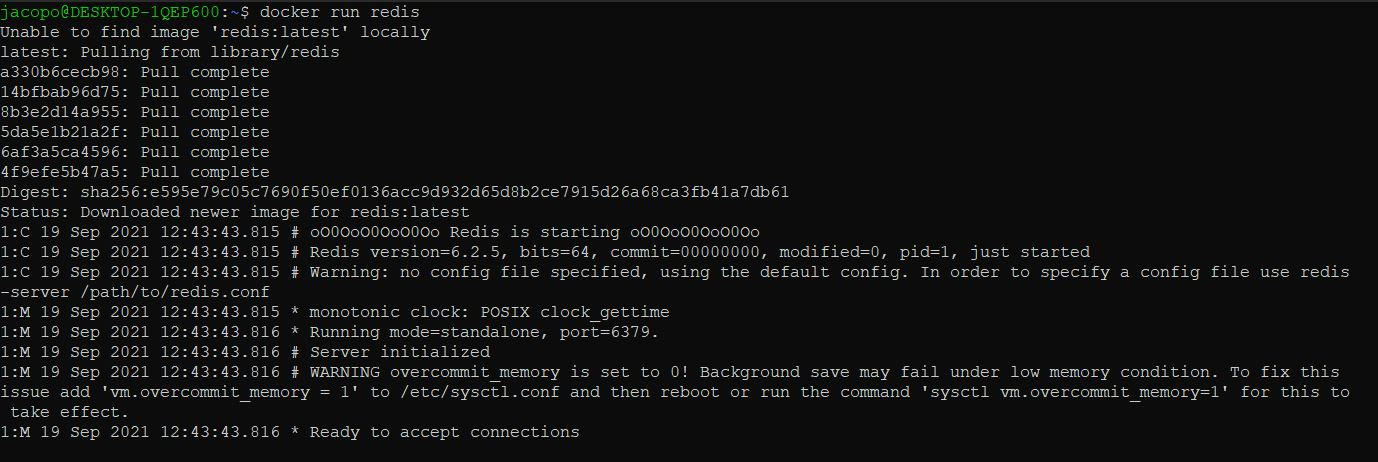
\includegraphics[scale=0.6]{img/006.jpg}
		\caption{docker non accessibile dall'esterno}
		\label{fig: 006}
	\end{center}
\end{figure}

Per questo dobbiamo lanciare \emph\textbf{{docker exec -it $<$container id$>$ $<$comando$>$}}, in questo modo diciamo che vogliamo eseguire un comando (exec) attraverso un input (-it) all'interno del container specificato.

\begin{figure}[h!]
	\begin{center}
		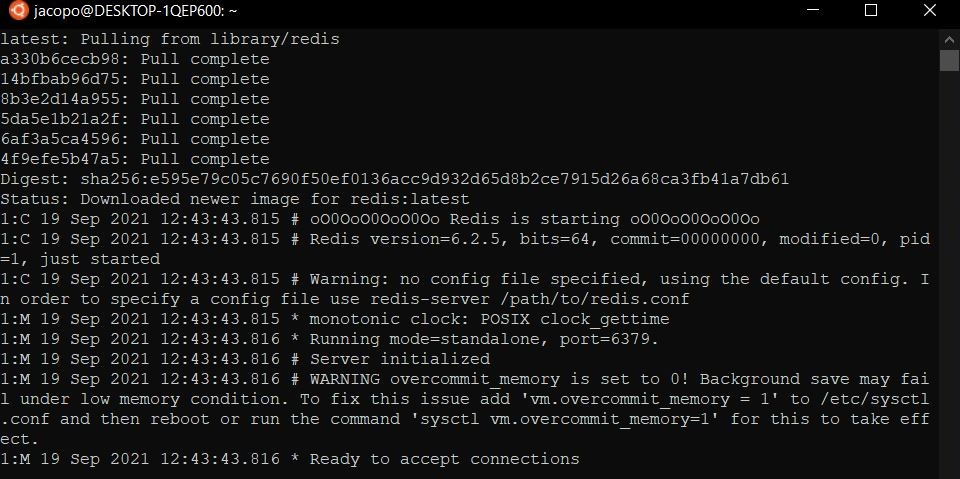
\includegraphics[scale=0.6]{img/007a.jpg}
		\caption{docker exec}
		\label{fig: 007a}
		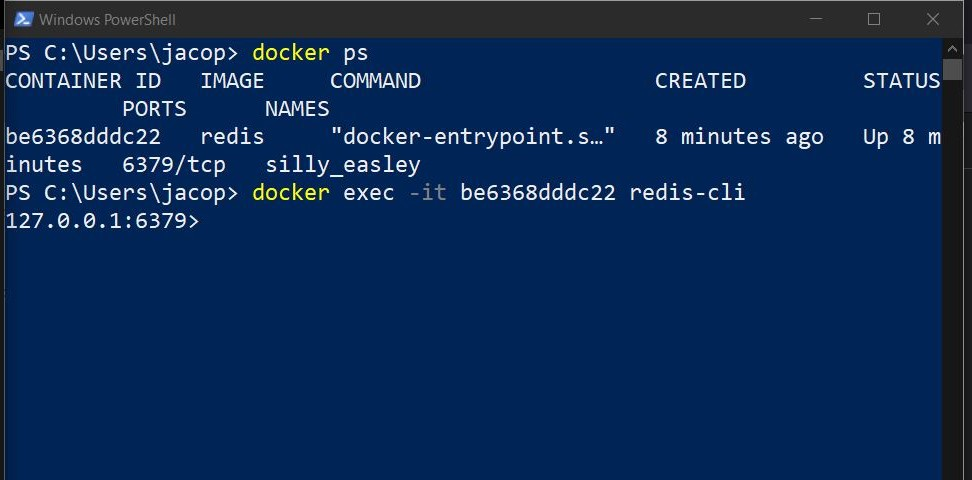
\includegraphics[scale=0.6]{img/007b.jpg}
		\caption{docker exec}
		\label{fig: 007b}
	\end{center}
\end{figure}

Senza -it non potremmo inserire alcun input. Ogni processo in un container ha tre stream (stdin, stdout, stderr). Attenzione, it è in realtà -i -t, nel primo stiamo dicendo ricevi l'input in stdin, -t segnala che si vuole un output leggibile.

\section{Aprire un prompt all'interno di un container}
\emph{\textbf{docker exec -it $<$container id$>$ sh}}, quel sh ci permette di aprire un terminale all'interno del container. Per uscire dal container \emph{ctrl + D}. \emph{\textbf{docker run -it $<$container id$>$ sh}} ottiene lo stesso risultato.

\section{Isolamento dei container}
Come è già stato detto un container ha il suo set di risorse e di memoria, questo vuole dire che i container non condividono nessuna informazione tra di loro.

\chapter{Creazione di un'immagine}
Dovremo creare un dockerfile. Immaginiamo di volere creare un'immagine che lancerà il redis server al suo avvio.

Prima di tutto creiamo una nuova cartella che conterrà i file, al suo interno creiamo un file chiamato \textbf{Dockerfile}, nessuna estensione. Al suo interno scriviamo un set di istruzioni:
\begin{lstlisting}
# Usare un'immagine esistente come base
FROM alpine

# Scaricare e installare una dipendenza
RUN apk add --update redis

# Dire all'immagine cosa fare al suo avvio come container
CMD ["redis-server"]
\end{lstlisting}

A questo punto scriviamo in console da dentro la cartella \emph{\textbf{docker build .}}, così verrà creata l'ìmmagine scaricando l'immagine di ALPINE, aggiornando il pacchetto redis e poi creare di default il comando redis-server.

\begin{figure}[h!]
	\begin{center}
		
\includegraphics[scale=0.6]{img/008.jpg}
		\caption{docker build}
		\label{fig: 008}
	\end{center}
\end{figure}

Il dockerfile contiene i vari step di creazione:
\begin{itemize}
	\item \textbf{FROM}: da che base
	\item \textbf{RUN}: eseguire un comando durante la preparazione dell'immagine
	\item \textbf{CMD}: cosa verrà lanciato all'avvio
\end{itemize}

\section{Cos'è un'immagine di base?}
Immaginiamo di dovere installare un programma senza avere un sistema operativo installato, quale sarebbe il primo passo? Installare un sistema operativo.

\section{E se modificassimo dockerfile?}
Nel caso di una modifica e di una successiva build docker userebbe la cache per partire dall'ultimo punto valido, in questo modo risparmierebbe tempo e risorse.

\section{Taggare un'immagine}
\emph{\textbf{docker build -t $<$docker ID/nome della repo/versione$>$}} permette di creare un tag per l'immagine. Solitamente questa è la sequenza usata, la versione tendenzialmente è "latest".

In questo modo potremmo usare un'immagine specifica tramite il tag usato, soprattutto se scaricato da docker hub.

\section{docker commit}
\emph{\textbf{docker commit -c 'CMD $<$comando$>$' $<$container id$>$}} fondamentalmente permette di creare un'immagine da un container attivo, fa ciò che fa un dockerfile ma dopo svariate modifiche dentro ad un container.

\chapter{docker compose}
\emph{\textbf{docker-compose}} permette di mettere in contatto più container senza dovere ripetere ogni volta gli stessi comandi. docker-compose sfrutta un file yml chiamato \textbf{docker-compose.yml}. 
\begin{lstlisting}
version: '3' # versione di docker-compose
services:
  redis-server:
    image: 'redis' # immagine su cui basarsi
  node-app:
    restart: always # riavvia automaticamente il servizio se si interrompe, on-failure si avvisa solo se l'exit code non è 0
    build: . # cartella da costruire
    ports:
      - "4081:8081" # porta dell'host:porta del container
\end{lstlisting}

docker-compose si occupa di creare questi due container all'interno dello stesso network, in questo modo non serve collegarli manualmente.

Invece di usare \emph{\textbf{docker run $<$immagine$>$}} ci basterà dire \emph{\textbf{docker-compose up}}.

Nel caso volessimo ricostruire le immagini ci basterebbe mettere \emph{\textbf{docker-compose up --build}}.


\emph{\textbf{docker-compose down}} spegne tutti i container assieme.

\emph{\textbf{docker-compose ps}} elenca i container attivi nella cartella.

\chapter{docker volumes}
I volumi sono semplicemente riferimenti a cartelle dell'host, in questo modo possiamo permettere un'interazione tra i due in maniera diretta. Il comando è \emph{\textbf{docker run -p $<$porta host$>$:$<$porta container$>$ -v $<$cartella relativa del volume$>$ -v \$($<$nome all-interno del volume$>$:/$<$cartella host$>$ $<$image ID$>$}}.
\end{document}